\documentclass[]{article}
\usepackage{lmodern}
\usepackage{amssymb,amsmath}
\usepackage{ifxetex,ifluatex}
\usepackage{fixltx2e} % provides \textsubscript
\ifnum 0\ifxetex 1\fi\ifluatex 1\fi=0 % if pdftex
  \usepackage[T1]{fontenc}
  \usepackage[utf8]{inputenc}
\else % if luatex or xelatex
  \ifxetex
    \usepackage{mathspec}
  \else
    \usepackage{fontspec}
  \fi
  \defaultfontfeatures{Ligatures=TeX,Scale=MatchLowercase}
\fi
% use upquote if available, for straight quotes in verbatim environments
\IfFileExists{upquote.sty}{\usepackage{upquote}}{}
% use microtype if available
\IfFileExists{microtype.sty}{%
\usepackage{microtype}
\UseMicrotypeSet[protrusion]{basicmath} % disable protrusion for tt fonts
}{}
\usepackage[margin=2.54cm]{geometry}
\usepackage{hyperref}
\hypersetup{unicode=true,
            pdftitle={Assignment 5: Data Visualization},
            pdfauthor={Keith Bollt},
            pdfborder={0 0 0},
            breaklinks=true}
\urlstyle{same}  % don't use monospace font for urls
\usepackage{color}
\usepackage{fancyvrb}
\newcommand{\VerbBar}{|}
\newcommand{\VERB}{\Verb[commandchars=\\\{\}]}
\DefineVerbatimEnvironment{Highlighting}{Verbatim}{commandchars=\\\{\}}
% Add ',fontsize=\small' for more characters per line
\usepackage{framed}
\definecolor{shadecolor}{RGB}{248,248,248}
\newenvironment{Shaded}{\begin{snugshade}}{\end{snugshade}}
\newcommand{\KeywordTok}[1]{\textcolor[rgb]{0.13,0.29,0.53}{\textbf{#1}}}
\newcommand{\DataTypeTok}[1]{\textcolor[rgb]{0.13,0.29,0.53}{#1}}
\newcommand{\DecValTok}[1]{\textcolor[rgb]{0.00,0.00,0.81}{#1}}
\newcommand{\BaseNTok}[1]{\textcolor[rgb]{0.00,0.00,0.81}{#1}}
\newcommand{\FloatTok}[1]{\textcolor[rgb]{0.00,0.00,0.81}{#1}}
\newcommand{\ConstantTok}[1]{\textcolor[rgb]{0.00,0.00,0.00}{#1}}
\newcommand{\CharTok}[1]{\textcolor[rgb]{0.31,0.60,0.02}{#1}}
\newcommand{\SpecialCharTok}[1]{\textcolor[rgb]{0.00,0.00,0.00}{#1}}
\newcommand{\StringTok}[1]{\textcolor[rgb]{0.31,0.60,0.02}{#1}}
\newcommand{\VerbatimStringTok}[1]{\textcolor[rgb]{0.31,0.60,0.02}{#1}}
\newcommand{\SpecialStringTok}[1]{\textcolor[rgb]{0.31,0.60,0.02}{#1}}
\newcommand{\ImportTok}[1]{#1}
\newcommand{\CommentTok}[1]{\textcolor[rgb]{0.56,0.35,0.01}{\textit{#1}}}
\newcommand{\DocumentationTok}[1]{\textcolor[rgb]{0.56,0.35,0.01}{\textbf{\textit{#1}}}}
\newcommand{\AnnotationTok}[1]{\textcolor[rgb]{0.56,0.35,0.01}{\textbf{\textit{#1}}}}
\newcommand{\CommentVarTok}[1]{\textcolor[rgb]{0.56,0.35,0.01}{\textbf{\textit{#1}}}}
\newcommand{\OtherTok}[1]{\textcolor[rgb]{0.56,0.35,0.01}{#1}}
\newcommand{\FunctionTok}[1]{\textcolor[rgb]{0.00,0.00,0.00}{#1}}
\newcommand{\VariableTok}[1]{\textcolor[rgb]{0.00,0.00,0.00}{#1}}
\newcommand{\ControlFlowTok}[1]{\textcolor[rgb]{0.13,0.29,0.53}{\textbf{#1}}}
\newcommand{\OperatorTok}[1]{\textcolor[rgb]{0.81,0.36,0.00}{\textbf{#1}}}
\newcommand{\BuiltInTok}[1]{#1}
\newcommand{\ExtensionTok}[1]{#1}
\newcommand{\PreprocessorTok}[1]{\textcolor[rgb]{0.56,0.35,0.01}{\textit{#1}}}
\newcommand{\AttributeTok}[1]{\textcolor[rgb]{0.77,0.63,0.00}{#1}}
\newcommand{\RegionMarkerTok}[1]{#1}
\newcommand{\InformationTok}[1]{\textcolor[rgb]{0.56,0.35,0.01}{\textbf{\textit{#1}}}}
\newcommand{\WarningTok}[1]{\textcolor[rgb]{0.56,0.35,0.01}{\textbf{\textit{#1}}}}
\newcommand{\AlertTok}[1]{\textcolor[rgb]{0.94,0.16,0.16}{#1}}
\newcommand{\ErrorTok}[1]{\textcolor[rgb]{0.64,0.00,0.00}{\textbf{#1}}}
\newcommand{\NormalTok}[1]{#1}
\usepackage{graphicx,grffile}
\makeatletter
\def\maxwidth{\ifdim\Gin@nat@width>\linewidth\linewidth\else\Gin@nat@width\fi}
\def\maxheight{\ifdim\Gin@nat@height>\textheight\textheight\else\Gin@nat@height\fi}
\makeatother
% Scale images if necessary, so that they will not overflow the page
% margins by default, and it is still possible to overwrite the defaults
% using explicit options in \includegraphics[width, height, ...]{}
\setkeys{Gin}{width=\maxwidth,height=\maxheight,keepaspectratio}
\IfFileExists{parskip.sty}{%
\usepackage{parskip}
}{% else
\setlength{\parindent}{0pt}
\setlength{\parskip}{6pt plus 2pt minus 1pt}
}
\setlength{\emergencystretch}{3em}  % prevent overfull lines
\providecommand{\tightlist}{%
  \setlength{\itemsep}{0pt}\setlength{\parskip}{0pt}}
\setcounter{secnumdepth}{0}
% Redefines (sub)paragraphs to behave more like sections
\ifx\paragraph\undefined\else
\let\oldparagraph\paragraph
\renewcommand{\paragraph}[1]{\oldparagraph{#1}\mbox{}}
\fi
\ifx\subparagraph\undefined\else
\let\oldsubparagraph\subparagraph
\renewcommand{\subparagraph}[1]{\oldsubparagraph{#1}\mbox{}}
\fi

%%% Use protect on footnotes to avoid problems with footnotes in titles
\let\rmarkdownfootnote\footnote%
\def\footnote{\protect\rmarkdownfootnote}

%%% Change title format to be more compact
\usepackage{titling}

% Create subtitle command for use in maketitle
\newcommand{\subtitle}[1]{
  \posttitle{
    \begin{center}\large#1\end{center}
    }
}

\setlength{\droptitle}{-2em}

  \title{Assignment 5: Data Visualization}
    \pretitle{\vspace{\droptitle}\centering\huge}
  \posttitle{\par}
    \author{Keith Bollt}
    \preauthor{\centering\large\emph}
  \postauthor{\par}
    \date{}
    \predate{}\postdate{}
  

\begin{document}
\maketitle

\subsection{OVERVIEW}\label{overview}

This exercise accompanies the lessons in Environmental Data Analytics
(ENV872L) on data wrangling.

\subsection{Directions}\label{directions}

\begin{enumerate}
\def\labelenumi{\arabic{enumi}.}
\tightlist
\item
  Change ``Student Name'' on line 3 (above) with your name.
\item
  Use the lesson as a guide. It contains code that can be modified to
  complete the assignment.
\item
  Work through the steps, \textbf{creating code and output} that fulfill
  each instruction.
\item
  Be sure to \textbf{answer the questions} in this assignment document.
  Space for your answers is provided in this document and is indicated
  by the ``\textgreater{}'' character. If you need a second paragraph be
  sure to start the first line with ``\textgreater{}''. You should
  notice that the answer is highlighted in green by RStudio.
\item
  When you have completed the assignment, \textbf{Knit} the text and
  code into a single PDF file. You will need to have the correct
  software installed to do this (see Software Installation Guide) Press
  the \texttt{Knit} button in the RStudio scripting panel. This will
  save the PDF output in your Assignments folder.
\item
  After Knitting, please submit the completed exercise (PDF file) to the
  dropbox in Sakai. Please add your last name into the file name (e.g.,
  ``Salk\_A04\_DataWrangling.pdf'') prior to submission.
\end{enumerate}

The completed exercise is due on Tuesday, 19 February, 2019 before class
begins.

\subsection{Set up your session}\label{set-up-your-session}

\begin{enumerate}
\def\labelenumi{\arabic{enumi}.}
\item
  Set up your session. Upload the NTL-LTER processed data files for
  chemistry/physics for Peter and Paul Lakes (tidy and gathered), the
  USGS stream gauge dataset, and the EPA Ecotox dataset for
  Neonicotinoids.
\item
  Make sure R is reading dates as date format, not something else (hint:
  remember that dates were an issue for the USGS gauge data).
\end{enumerate}

\begin{Shaded}
\begin{Highlighting}[]
\CommentTok{#1}
\KeywordTok{library}\NormalTok{(tidyverse)}
\end{Highlighting}
\end{Shaded}

\begin{verbatim}
## Warning: package 'tidyverse' was built under R version 3.5.2
\end{verbatim}

\begin{verbatim}
## -- Attaching packages --------------------------------------------------------------------------------- tidyverse 1.2.1 --
\end{verbatim}

\begin{verbatim}
## v ggplot2 3.1.0     v purrr   0.2.5
## v tibble  1.4.2     v dplyr   0.7.8
## v tidyr   0.8.2     v stringr 1.3.1
## v readr   1.3.1     v forcats 0.3.0
\end{verbatim}

\begin{verbatim}
## Warning: package 'ggplot2' was built under R version 3.5.2
\end{verbatim}

\begin{verbatim}
## Warning: package 'tibble' was built under R version 3.5.2
\end{verbatim}

\begin{verbatim}
## Warning: package 'tidyr' was built under R version 3.5.2
\end{verbatim}

\begin{verbatim}
## Warning: package 'readr' was built under R version 3.5.2
\end{verbatim}

\begin{verbatim}
## Warning: package 'purrr' was built under R version 3.5.2
\end{verbatim}

\begin{verbatim}
## Warning: package 'dplyr' was built under R version 3.5.2
\end{verbatim}

\begin{verbatim}
## Warning: package 'stringr' was built under R version 3.5.2
\end{verbatim}

\begin{verbatim}
## Warning: package 'forcats' was built under R version 3.5.2
\end{verbatim}

\begin{verbatim}
## -- Conflicts ------------------------------------------------------------------------------------ tidyverse_conflicts() --
## x dplyr::filter() masks stats::filter()
## x dplyr::lag()    masks stats::lag()
\end{verbatim}

\begin{Shaded}
\begin{Highlighting}[]
\KeywordTok{library}\NormalTok{(ggplot2)}
\NormalTok{lake.chem.nutrients.tidy <-}\StringTok{ }
\StringTok{  }\KeywordTok{read.csv}\NormalTok{(}\StringTok{"V:/ENV_872_Project_Directory/Data/Processed/NTL-LTER_Lake_Chemistry_Nutrients_PeterPaul_Processed.csv"}\NormalTok{)}
\NormalTok{lake.chem.nutrients.gathered <-}
\StringTok{  }\KeywordTok{read.csv}\NormalTok{(}\StringTok{"V:/ENV_872_Project_Directory/Data/Processed/NTL-LTER_Lake_Nutrients_PeterPaulGathered_Processed.csv"}\NormalTok{)}
\NormalTok{usgs.A05 <-}\StringTok{ }
\StringTok{  }\KeywordTok{read.csv}\NormalTok{(}\StringTok{"V:/ENV_872_Project_Directory/Data/raw/USGS_Site02085000_Flow_Raw.csv"}\NormalTok{)}
\NormalTok{neonicotinoids.A05 <-}
\StringTok{   }\KeywordTok{read.csv}\NormalTok{(}\StringTok{"V:/ENV_872_Project_Directory/Data/raw/ECOTOX_Neonicotinoids_Mortality_raw.csv"}\NormalTok{)}

\CommentTok{#2}
\KeywordTok{data.class}\NormalTok{(usgs.A05}\OperatorTok{$}\NormalTok{datetime)}
\end{Highlighting}
\end{Shaded}

\begin{verbatim}
## [1] "factor"
\end{verbatim}

\begin{Shaded}
\begin{Highlighting}[]
\NormalTok{usgs.A05}\OperatorTok{$}\NormalTok{datetime <-}\StringTok{ }\KeywordTok{as.Date}\NormalTok{(usgs.A05}\OperatorTok{$}\NormalTok{datetime, }\DataTypeTok{format =} \StringTok{"%m/%d/%y"}\NormalTok{)}
\NormalTok{usgs.A05}\OperatorTok{$}\NormalTok{datetime <-}\StringTok{ }\KeywordTok{format}\NormalTok{(usgs.A05}\OperatorTok{$}\NormalTok{datetime, }\StringTok{"%y%m%d"}\NormalTok{) }
\NormalTok{create.early.dates <-}\StringTok{ }\NormalTok{(}\ControlFlowTok{function}\NormalTok{(d) \{}
       \KeywordTok{paste0}\NormalTok{(}\KeywordTok{ifelse}\NormalTok{(d }\OperatorTok{>}\StringTok{ }\DecValTok{181231}\NormalTok{,}\StringTok{"19"}\NormalTok{,}\StringTok{"20"}\NormalTok{),d)}
\NormalTok{       \}) }
\NormalTok{usgs.A05}\OperatorTok{$}\NormalTok{datetime <-}\StringTok{ }\KeywordTok{create.early.dates}\NormalTok{(usgs.A05}\OperatorTok{$}\NormalTok{datetime)}
\NormalTok{usgs.A05}\OperatorTok{$}\NormalTok{datetime <-}\StringTok{ }\KeywordTok{as.Date}\NormalTok{(usgs.A05}\OperatorTok{$}\NormalTok{datetime, }\DataTypeTok{format =} \StringTok{"%Y%m%d"}\NormalTok{)}


\KeywordTok{data.class}\NormalTok{(lake.chem.nutrients.tidy}\OperatorTok{$}\NormalTok{sampledate)}
\end{Highlighting}
\end{Shaded}

\begin{verbatim}
## [1] "factor"
\end{verbatim}

\begin{Shaded}
\begin{Highlighting}[]
\NormalTok{lake.chem.nutrients.tidy}\OperatorTok{$}\NormalTok{sampledate <-}\StringTok{ }\KeywordTok{as.Date}\NormalTok{(lake.chem.nutrients.tidy}\OperatorTok{$}\NormalTok{sampledate, }\DataTypeTok{format =} \StringTok{"%Y-%m-%d"}\NormalTok{)}
\KeywordTok{data.class}\NormalTok{(lake.chem.nutrients.gathered}\OperatorTok{$}\NormalTok{sampledate)}
\end{Highlighting}
\end{Shaded}

\begin{verbatim}
## [1] "factor"
\end{verbatim}

\begin{Shaded}
\begin{Highlighting}[]
\NormalTok{lake.chem.nutrients.gathered}\OperatorTok{$}\NormalTok{sampledate <-}\StringTok{ }\KeywordTok{as.Date}\NormalTok{(lake.chem.nutrients.gathered}\OperatorTok{$}\NormalTok{sampledate, }\DataTypeTok{format =} \StringTok{"%Y-%m-%d"}\NormalTok{)}
\end{Highlighting}
\end{Shaded}

\subsection{Define your theme}\label{define-your-theme}

\begin{enumerate}
\def\labelenumi{\arabic{enumi}.}
\setcounter{enumi}{2}
\tightlist
\item
  Build a theme and set it as your default theme.
\end{enumerate}

\begin{Shaded}
\begin{Highlighting}[]
\CommentTok{#3}
\NormalTok{mytheme <-}\StringTok{ }\KeywordTok{theme_classic}\NormalTok{(}\DataTypeTok{base_size =} \FloatTok{12.92}\NormalTok{)}\OperatorTok{+}
\StringTok{  }\KeywordTok{theme}\NormalTok{(}\DataTypeTok{axis.text =} \KeywordTok{element_text}\NormalTok{(}\DataTypeTok{color =} \StringTok{"blue"}\NormalTok{),}
  \DataTypeTok{legend.position =} \StringTok{"top"}\NormalTok{)}
\end{Highlighting}
\end{Shaded}

\subsection{Create graphs}\label{create-graphs}

For numbers 4-7, create graphs that follow best practices for data
visualization. To make your graphs ``pretty,'' ensure your theme, color
palettes, axes, and legends are edited to your liking.

Hint: a good way to build graphs is to make them ugly first and then
create more code to make them pretty.

\begin{enumerate}
\def\labelenumi{\arabic{enumi}.}
\setcounter{enumi}{3}
\tightlist
\item
  {[}NTL-LTER{]} Plot total phosphorus by phosphate, with separate
  aesthetics for Peter and Paul lakes. Add a line of best fit and color
  it black.
\end{enumerate}

\begin{Shaded}
\begin{Highlighting}[]
\CommentTok{#4}
\NormalTok{phosphorus_vs_phosphate <-}\StringTok{ }\KeywordTok{ggplot}\NormalTok{(lake.chem.nutrients.tidy, }\KeywordTok{aes}\NormalTok{(}\DataTypeTok{x =}\NormalTok{ po4, }\DataTypeTok{y =}\NormalTok{ tp_ug, }\DataTypeTok{color =}\NormalTok{ depth, }\DataTypeTok{shape =}\NormalTok{ lakename))}\OperatorTok{+}
\StringTok{  }\KeywordTok{geom_point}\NormalTok{()}\OperatorTok{+}
\StringTok{  }\KeywordTok{xlab}\NormalTok{(}\KeywordTok{expression}\NormalTok{ (}\StringTok{"Phosphate (μg/L)"}\NormalTok{))}\OperatorTok{+}
\StringTok{  }\KeywordTok{ylab}\NormalTok{(}\KeywordTok{expression}\NormalTok{ (}\StringTok{"Total Phosphorus (μg/L)"}\NormalTok{))}\OperatorTok{+}
\StringTok{  }\KeywordTok{labs}\NormalTok{(}\DataTypeTok{shape =} \StringTok{"Lake"}\NormalTok{)}\OperatorTok{+}
\StringTok{  }\KeywordTok{geom_smooth}\NormalTok{(}\DataTypeTok{method =}\NormalTok{ lm, }\DataTypeTok{color =} \StringTok{"black"}\NormalTok{)}

\KeywordTok{print}\NormalTok{(phosphorus_vs_phosphate)}
\end{Highlighting}
\end{Shaded}

\begin{verbatim}
## Warning: Removed 22309 rows containing non-finite values (stat_smooth).
\end{verbatim}

\begin{verbatim}
## Warning: Removed 22309 rows containing missing values (geom_point).
\end{verbatim}

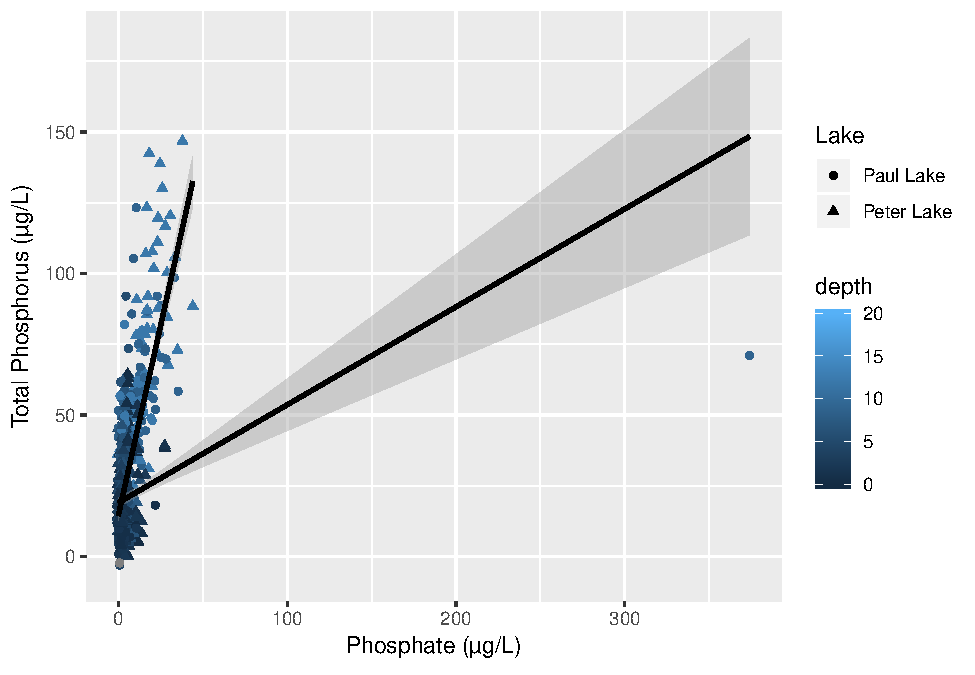
\includegraphics{A05_DataVisualization_files/figure-latex/unnamed-chunk-3-1.pdf}

\begin{enumerate}
\def\labelenumi{\arabic{enumi}.}
\setcounter{enumi}{4}
\tightlist
\item
  {[}NTL-LTER{]} Plot nutrients by date for Peter Lake, with separate
  colors for each depth. Facet your graph by the nutrient type.
\end{enumerate}

\begin{Shaded}
\begin{Highlighting}[]
\CommentTok{#5}
\NormalTok{graph5 <-}\StringTok{ }\KeywordTok{ggplot}\NormalTok{(}\KeywordTok{subset}\NormalTok{(lake.chem.nutrients.gathered, lakename }\OperatorTok{==}\StringTok{ "Peter Lake"}\NormalTok{), }\KeywordTok{aes}\NormalTok{(}\DataTypeTok{x=}\NormalTok{ sampledate, }\DataTypeTok{y=}\NormalTok{ concentration, }\DataTypeTok{color =}\NormalTok{ depth))}\OperatorTok{+}
\StringTok{  }\KeywordTok{geom_point}\NormalTok{()}\OperatorTok{+}
\StringTok{  }\KeywordTok{ylab}\NormalTok{(}\KeywordTok{expression}\NormalTok{(}\StringTok{"Concentration (μg/L)"}\NormalTok{))}\OperatorTok{+}
\StringTok{  }\KeywordTok{xlab}\NormalTok{(}\KeywordTok{expression}\NormalTok{(}\StringTok{"Date"}\NormalTok{))}
 
  
\KeywordTok{print}\NormalTok{(graph5)}
\end{Highlighting}
\end{Shaded}

\includegraphics{A05_DataVisualization_files/figure-latex/unnamed-chunk-4-1.pdf}

\begin{Shaded}
\begin{Highlighting}[]
\KeywordTok{facet_grid}\NormalTok{(concentration }\OperatorTok{~}\StringTok{ }\NormalTok{nutrient)}
\end{Highlighting}
\end{Shaded}

\begin{verbatim}
## <ggproto object: Class FacetGrid, Facet, gg>
##     compute_layout: function
##     draw_back: function
##     draw_front: function
##     draw_labels: function
##     draw_panels: function
##     finish_data: function
##     init_scales: function
##     map_data: function
##     params: list
##     setup_data: function
##     setup_params: function
##     shrink: TRUE
##     train_scales: function
##     vars: function
##     super:  <ggproto object: Class FacetGrid, Facet, gg>
\end{verbatim}

\begin{enumerate}
\def\labelenumi{\arabic{enumi}.}
\setcounter{enumi}{5}
\tightlist
\item
  {[}USGS gauge{]} Plot discharge by date. Create two plots, one with
  the points connected with geom\_line and one with the points connected
  with geom\_smooth (hint: do not use method = ``lm''). Place these
  graphs on the same plot (hint: ggarrange or something similar)
\end{enumerate}

\begin{Shaded}
\begin{Highlighting}[]
\CommentTok{#6}
\NormalTok{Discharge_v_date_smooth <-}\StringTok{ }\KeywordTok{ggplot}\NormalTok{(usgs.A05, }\KeywordTok{aes}\NormalTok{(}\DataTypeTok{x =}\NormalTok{ datetime, }\DataTypeTok{y =}\NormalTok{ X165986_00060_}\DecValTok{00001}\NormalTok{))}\OperatorTok{+}
\StringTok{  }\KeywordTok{geom_point}\NormalTok{()}\OperatorTok{+}
\StringTok{  }\KeywordTok{geom_smooth}\NormalTok{()}\OperatorTok{+}
\StringTok{  }\KeywordTok{xlab}\NormalTok{(}\KeywordTok{expression}\NormalTok{(}\StringTok{"Date"}\NormalTok{))}\OperatorTok{+}
\StringTok{  }\KeywordTok{ylab}\NormalTok{(}\KeywordTok{expression}\NormalTok{(}\StringTok{"Discharge in CFS"}\NormalTok{))}
\KeywordTok{print}\NormalTok{(Discharge_v_date_smooth)}
\end{Highlighting}
\end{Shaded}

\begin{verbatim}
## `geom_smooth()` using method = 'gam' and formula 'y ~ s(x, bs = "cs")'
\end{verbatim}

\begin{verbatim}
## Warning: Removed 5113 rows containing non-finite values (stat_smooth).
\end{verbatim}

\begin{verbatim}
## Warning: Removed 5113 rows containing missing values (geom_point).
\end{verbatim}

\includegraphics{A05_DataVisualization_files/figure-latex/unnamed-chunk-5-1.pdf}

\begin{Shaded}
\begin{Highlighting}[]
\NormalTok{Discharge_v_date_line <-}\StringTok{ }\KeywordTok{ggplot}\NormalTok{(usgs.A05, }\KeywordTok{aes}\NormalTok{(}\DataTypeTok{x =}\NormalTok{ datetime, }\DataTypeTok{y =}\NormalTok{ X165986_00060_}\DecValTok{00001}\NormalTok{))}\OperatorTok{+}
\StringTok{  }\KeywordTok{geom_point}\NormalTok{()}\OperatorTok{+}
\StringTok{  }\KeywordTok{geom_line}\NormalTok{()}\OperatorTok{+}
\StringTok{  }\KeywordTok{xlab}\NormalTok{(}\KeywordTok{expression}\NormalTok{(}\StringTok{"Date"}\NormalTok{))}\OperatorTok{+}
\StringTok{  }\KeywordTok{ylab}\NormalTok{(}\KeywordTok{expression}\NormalTok{(}\StringTok{"Discharge in CFS"}\NormalTok{))}
\KeywordTok{print}\NormalTok{(Discharge_v_date_line)}
\end{Highlighting}
\end{Shaded}

\begin{verbatim}
## Warning: Removed 5113 rows containing missing values (geom_point).
\end{verbatim}

\includegraphics{A05_DataVisualization_files/figure-latex/unnamed-chunk-5-2.pdf}

\begin{Shaded}
\begin{Highlighting}[]
\KeywordTok{library}\NormalTok{(ggpubr)}
\end{Highlighting}
\end{Shaded}

\begin{verbatim}
## Warning: package 'ggpubr' was built under R version 3.5.2
\end{verbatim}

\begin{verbatim}
## Loading required package: magrittr
\end{verbatim}

\begin{verbatim}
## Warning: package 'magrittr' was built under R version 3.5.2
\end{verbatim}

\begin{verbatim}
## 
## Attaching package: 'magrittr'
\end{verbatim}

\begin{verbatim}
## The following object is masked from 'package:purrr':
## 
##     set_names
\end{verbatim}

\begin{verbatim}
## The following object is masked from 'package:tidyr':
## 
##     extract
\end{verbatim}

\begin{Shaded}
\begin{Highlighting}[]
\KeywordTok{ggarrange}\NormalTok{(Discharge_v_date_smooth, Discharge_v_date_line)}
\end{Highlighting}
\end{Shaded}

\begin{verbatim}
## `geom_smooth()` using method = 'gam' and formula 'y ~ s(x, bs = "cs")'
\end{verbatim}

\begin{verbatim}
## Warning: Removed 5113 rows containing non-finite values (stat_smooth).

## Warning: Removed 5113 rows containing missing values (geom_point).

## Warning: Removed 5113 rows containing missing values (geom_point).
\end{verbatim}

\includegraphics{A05_DataVisualization_files/figure-latex/unnamed-chunk-5-3.pdf}
Question: How do these two types of lines affect your interpretation of
the data?

\begin{quote}
Answer: The gg\_smooth plot creates a trendline, and suggests a temporal
trend over time (whether or not a strongly correlated trend actually
exists). It also draws a trend right through the years for which no data
exists. On the other hand, the gg\_line plot connects each point to the
previous point. Among other things, this has the effect of blurring out
densly plotted points because they are covered by the line itself, and
also disguising statistical outliers as being more typical of the
dataset.
\end{quote}

\begin{enumerate}
\def\labelenumi{\arabic{enumi}.}
\setcounter{enumi}{6}
\tightlist
\item
  {[}ECOTOX Neonicotinoids{]} Plot the concentration, divided by
  chemical name. Choose a geom that accurately portrays the distribution
  of data points.
\end{enumerate}

\begin{Shaded}
\begin{Highlighting}[]
\CommentTok{#7 }

\NormalTok{neonic <-}\StringTok{ }\KeywordTok{ggplot}\NormalTok{(}\KeywordTok{subset}\NormalTok{(neonicotinoids.A05, Conc..Units..Std. }\OperatorTok{==}\StringTok{ "AL mg/L"}\NormalTok{), }\KeywordTok{aes}\NormalTok{(}\DataTypeTok{x =}\NormalTok{ Chemical.Name, }\DataTypeTok{y =}\NormalTok{ Conc..Mean..Std., }\DataTypeTok{fill =} \KeywordTok{as.factor}\NormalTok{(Chemical.Name)))}\OperatorTok{+}
\StringTok{  }\KeywordTok{geom_bar}\NormalTok{(}\DataTypeTok{stat =} \StringTok{"identity"}\NormalTok{, }\DataTypeTok{position =} \StringTok{"dodge"}\NormalTok{)}\OperatorTok{+}
\StringTok{  }\KeywordTok{xlab}\NormalTok{(}\KeywordTok{expression}\NormalTok{(}\StringTok{"Chemical Name"}\NormalTok{))}\OperatorTok{+}
\StringTok{  }\KeywordTok{ylab}\NormalTok{(}\KeywordTok{expression}\NormalTok{(}\StringTok{"Concentration (mg/L)"}\NormalTok{))}

\KeywordTok{print}\NormalTok{(neonic)}
\end{Highlighting}
\end{Shaded}

\includegraphics{A05_DataVisualization_files/figure-latex/unnamed-chunk-6-1.pdf}


\end{document}
